\graphicspath{{./figures}}

\section{Range}

Line-of-sight range tests were conducted. Both antennas were manually positioning to determine the system's capabilities. Various measurements were done at the originally designed parameters (e.g. SF 8, CR 4/6, 500 kHz) and with automatic gain control (AGC). The resulting \textit{received signal strength indicator} (RSSI), signal-to-noise (SNR) ratio, and packet reception rate (PRR i.e. percentage of non-corrupted packets received) was recorded. For the unfamiliar reader, the highest (best) theoretical RSSI is 0 dB, and the minimum SNR for SF 8 is -10 dB (LoRa is capable of demodulating negative signal-to-noise ratios).

\begin{table}[!htb]
  \centering
  \renewcommand{\arraystretch}{1.2}
  \hspace*{-1.5cm}
  \begin{tabular}{ |c|c|c|c|c| }
  \hline
  \textbf{Test No.}         & \textbf{Range}        & \textbf{GS Location}      & \textbf{PQ Location}      & \textbf{Comments} \\ 
  \hline
  1                         
  & 1.4 km  
  & Firgrove Way
  & M3 Bridge 
  & \\ \hline
  2
  & 4.6 km  
  & Constantia
  & Silvermine
  & Cloudy conditions \\ \hline
  3
  & 9.7 km  
  & Boys' Drive
  & Simon's Town
  & \\ \hline
  4
  & 34.5 km  
  & Steenbras
  & Simon's Town
  & \\ \hline
  5
  & 49 km  
  & Takara Stellenbosch  
  & Silvermine
  & Optimal transmitter placement uncertainty \\ \hline
  \end{tabular}
  \caption{Range Test Locations}
  \label{tab:rangeTestLocations}
\end{table}

Tests were done in locations around the Western Cape. These locations are described in Table \ref{tab:rangeTestLocations} and mapped out in Appendix \ref{sec:appendix_range}. The first primitive test (which is not listed) was a 300 m test on Coetzenburg field in Stellenbosch. The performance of this test was found to be low compared to subsequent tests, with an RSSI of around -92 dBm recorded. It is assumed that ground bounce was the major contributing factor to this, due to the low operating frequency of the system (around 430 MHz) and the close proximity (around 1m) the antennas had to the ground.

The final results are plotted as a function of distance in Figures \ref{fig:rangeRssi} and \ref{fig:rangeSnr}, with a logarithmic curve fit. All measurements were taken as an average of at least 10 consecutive samples. The dipole was both horizontally and vertically placed. The packet contents were verified using a packet ID, the GPS location of the transmitter, as well as inspecting whether a CRC (Cyclic Redundancy Check) error had occurred. If any of these were incorrect, the packet was considered "missed".

\begin{figure}[!htb]
  \centering
  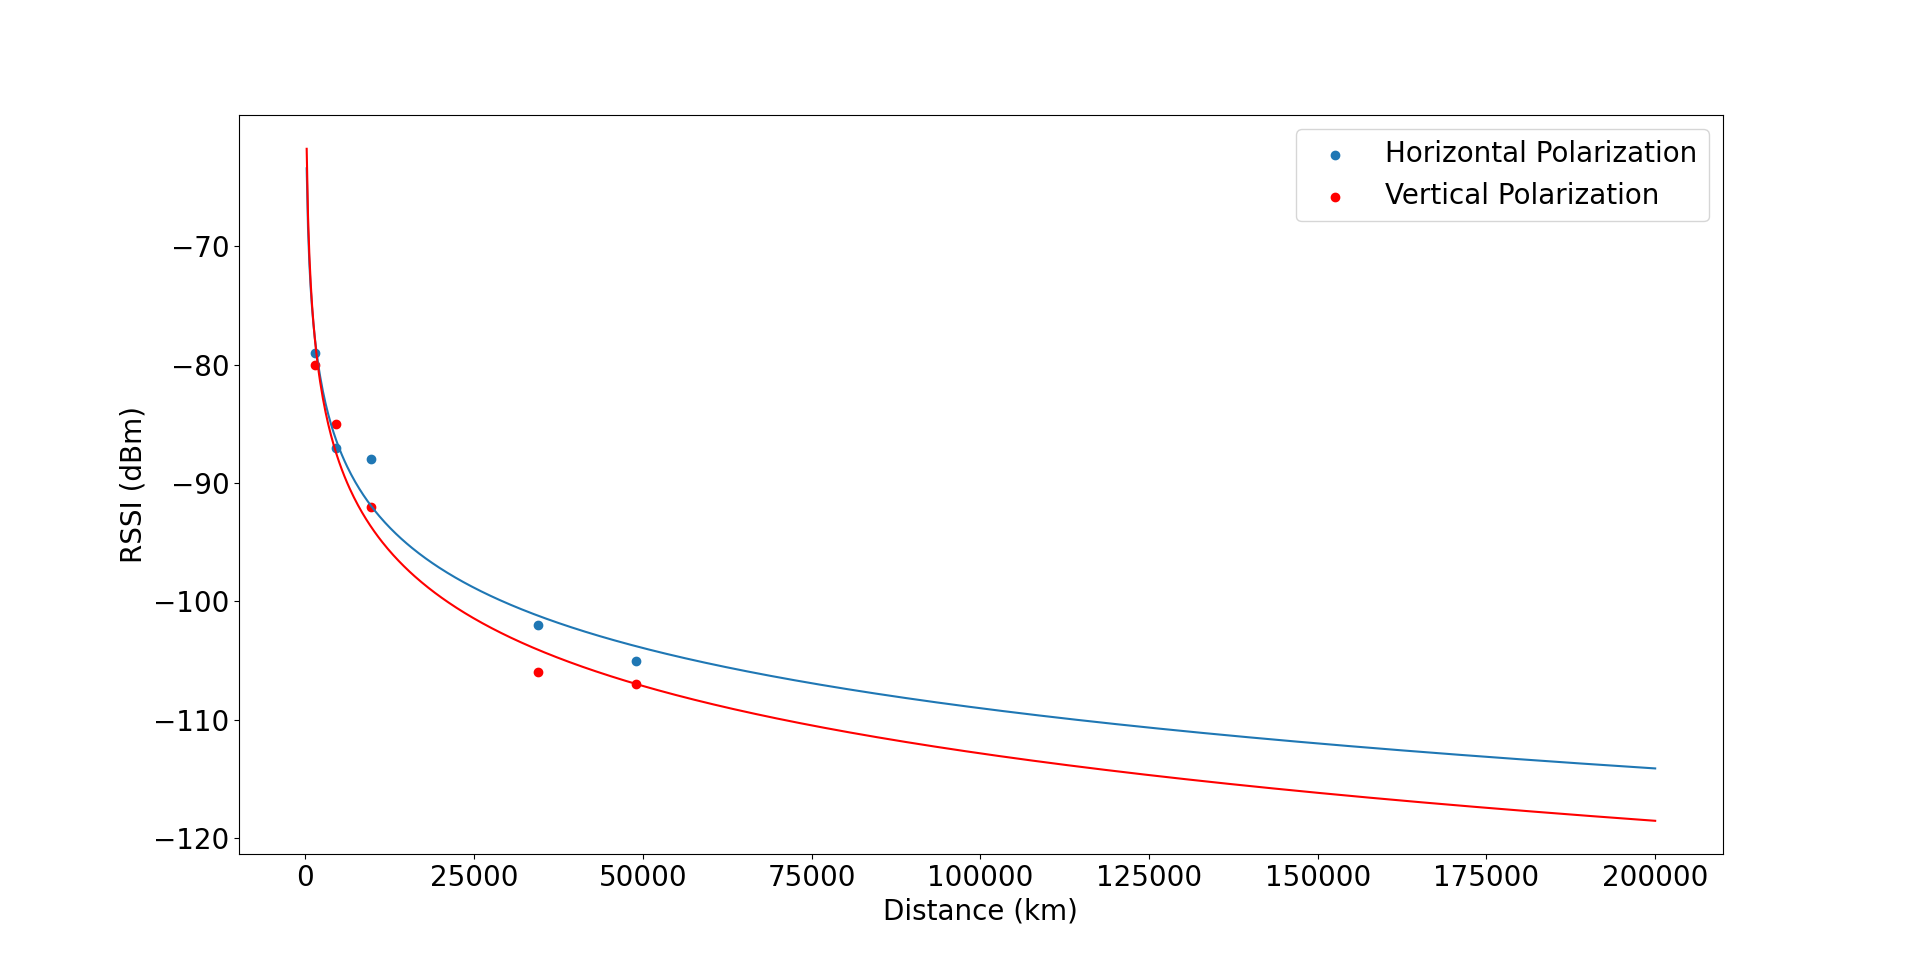
\includegraphics[width=0.9\textwidth]{rangeRssi}
  \caption{Measured RSSI vs Distance}
  \label{fig:rangeRssi}
\end{figure}

\begin{figure}[!htb]
  \centering
  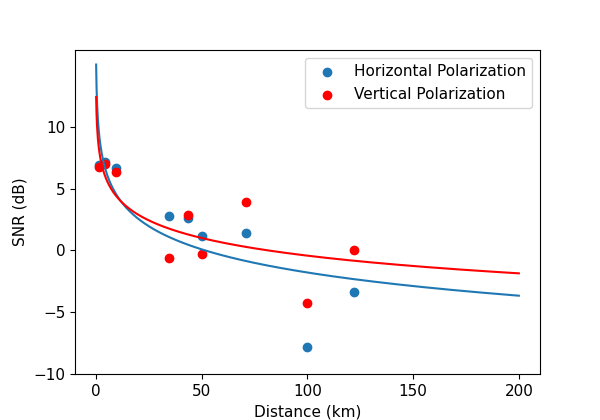
\includegraphics[width=0.9\textwidth]{rangeSnr}
  \caption{Measured SNR vs Distance}
  \label{fig:rangeSnr}
\end{figure}

The data shows that the system would successfully meet the 110 km range requirement. No CRC errors were found once the system was in steady state for all tests. The final test at 50 km recorded an RSSI of around -107 dBm for the vertically polarized case. The predicted RSSI for vertical polarization at 125 km is around -114 dBm, whereas the receiver sensitivity is as low as -119 dBm, indicating a 5 dB margin. It should be noted that the SNR logarithmic fit is not considered reliable, since the receiver appears to adjust the gain to keep the SNR around 7.5 dB for closer distances. However, the RSSI appears to follow a logarithmic curve as predicted by the free space path loss formulae. \textcolor{red}{I hope to still do a final 110 km range test from table mountain up the west coast to fully verify my design}